\subsubsection{One-zone collapse test}
\label{sec.tests.1-zone}

The one-zone collapse test simulates the collapse of a
self-gravitating gas cloud using a semi-analytic model for the
evolution of gas density and adiabatic heat input as a function of
time.  It is designed to test the chemistry and cooling modules over a
wide range in densities and over physically motivated timescales.
Because this test disables the hydrodynamic and gravity solvers and
uses a simple model for the density evolution, it is far faster than
running a true collapse simulation.  The density evolution is based on
the self-similar Larson-Penston \citep{1969MNRAS.145..271L,
1969MNRAS.144..425P} solution for isothermal collapse with a
modification to account for the efficiency with which the heat
introduced by compression can be radiated away
\citep{1983ApJ...265.1047Y}.  Our implementation, described briefly
here, follows the work of \citet{2005ApJ...626..627O}, and we direct
the interested reader to this paper for further details.  The
evolution of the gas density, $\rho$, is given by

\begin{equation}
\frac{d\rho}{dt} = \frac{\rho}{t_{\rm col}},
\end{equation}

where the collapse timescale, $t_{\rm col}$, is

\begin{equation} \label{eqn.tcol}
t_{\rm col} = \frac{t_{\rm dyn}}{\sqrt{1 - f}},
\end{equation}
In this equation, $t_{\rm dyn}$ is the dynamical time and is expressed as
\begin{equation}
t_{\rm dyn} = \sqrt{\frac{3 \pi}{32 G \rho}}.
\end{equation}

with G being the gravitational constant. \mqk{Instead of explaining what $G$ is here, would it make sense to have a table at the beginning of the paper listing all the natural constants and variable symbols that are used throughout the paper?} The collapse timescale is
altered from the dynamical time by a factor $1/\sqrt{1-f}$ in Equation
\ref{eqn.tcol}, which is an approximation of the ratio of the gas
pressure to the force of gravity.  The value of $f$ depends on the
effective adiabatic index, $\gamma_{\rm ef} \equiv (\partial \ln p
/ \partial \ln \rho)$, which we linearly extrapolate
from derivative values at the two previous timesteps.  For the value
of $f$ in this test problem, we use the piecewise function of
\citet{2005ApJ...626..627O}, given by

\begin{equation}
f = \left\{
  \begin{array}{ll}
  0, & \gamma_{\rm ef} < 0.83,\\
  0.6 + 2.5 (\gamma_{\rm ef} - 1) - 6.0 (\gamma_{\rm ef} - 1)^{2}, & 0.83 <
  \gamma_{\rm ef} < 1,\\
  1.0 + 0.2 (\gamma_{\rm ef} - 4/3) - 2.9 (\gamma_{\rm ef} - 4/3)^{2}, & \gamma_{\rm ef} > 1.
\end{array} \right.
\end{equation}

The specific energy evolves as

\begin{equation}
\frac{de}{dt} = -p \frac{d}{dt} \frac{1}{\rho} - \Lambda,
\end{equation}

where $\Lambda$ is the cooling rate in units of erg s$^{-1}$ g$^{-1}$
and energy, temperature, density, and pressure are related by the
ideal gas law.  Figure \ref{fig.onezone} shows an example of the
one-zone collapse test performed with an initial number density of 1
hydrogen atom per cm$^{-3}$ and an initial temperature of 100 K using
the 12 species chemistry network with H, D, and He species and metal
cooling rates calculated with the \texttt{Cloudy} code.  The effects
of metal cooling can be clearly seen; as the metallicity increases
from zero to $10^{-2}$~Z$_\odot$, the gas rapidly and significantly
deviates from the primordial result (black line).  Our primordial
results compare very well to those shown in
\citet{2005ApJ...626..627O}; however, we use a different metal cooling
method, so the lines describing the evolution of the
metal-enriched gas are not directly comparable.

\begin{figure}
  \begin{center}
    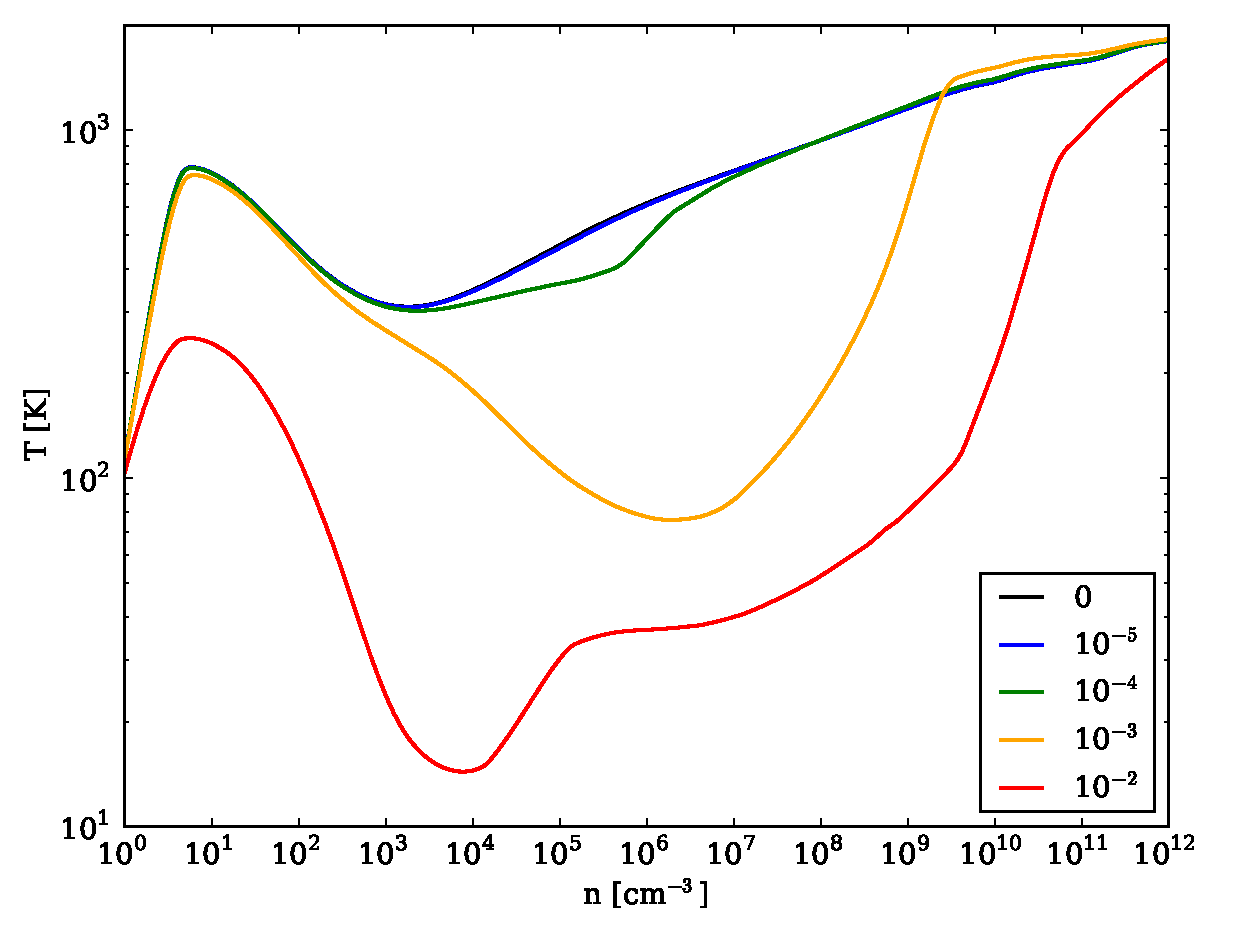
\includegraphics[width=1.0\textwidth]{figures/OneZoneCollapseTest.eps}
  \end{center}
  \caption{Evolution of temperature versus number density for a
one-zone collapse test for gas at metallicities from 0 to 10$^{-2}
Z_{\odot}$.  This test is based on the results of
\citet{2005ApJ...626..627O}, and approximates the collapse of a
self-gravitating, cooling gas cloud.  This test problem uses \enzo's
primordial chemistry network with tabulated metal cooling rates
calculated with the \texttt{Cloudy} code, and compares favorably to
the results of \citet{2005ApJ...626..627O}.}
  \label{fig.onezone}
\end{figure}
